


\documentclass[crop,tikz]{standalone}% 'crop' is the default for v1.0, before it was 'preview'
%\usetikzlibrary{...}% tikz package already loaded by 'tikz' option
\usetikzlibrary{trees}
\usetikzlibrary{shapes}
\usetikzlibrary{trees}
\usetikzlibrary{shapes}
\usetikzlibrary{matrix, fit}
\usetikzlibrary{arrows}
\usetikzlibrary{shapes}

\usepackage{bm}

\begin{document}



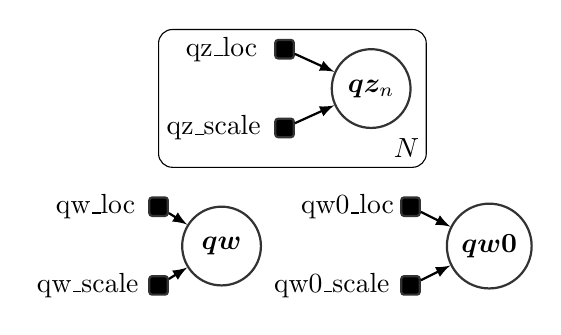
\begin{tikzpicture}

\tikzstyle{hidden}=[circle, minimum size = 10mm, thick, draw =black!80, node distance = 16mm]
\tikzstyle{observed}=[circle, minimum size = 10mm, thick, draw =black!80, node distance = 16mm, fill=gray!50]
\tikzstyle{trainvar}=[rectangle, minimum size = 2mm, rounded corners=1pt, thick, draw =black!80, node distance = 16mm, fill=black]


\tikzstyle{connect}=[-latex, thick]



\node[hidden] (qzn) at (0.3,1.5)  {$\bm{qz}_n$};
\node[trainvar] (qzloc) at (-0.8, 2)  {};
\node[trainvar] (qzscale) at (-0.8,1.0)  {};
\node[] () at (-1.6, 2)  {qz\_loc};
\node[] () at (-1.7,1.0)  {qz\_scale};




\node[hidden] (qw) at (-1.6,-0.5)  {$\bm{qw}$};
\node[trainvar] (qwloc) at (-2.4, 0)  {};
\node[trainvar] (qwscale) at (-2.4,-1.0)  {};
\node[] () at (-3.2, 0)  {qw\_loc};
\node[] () at (-3.3,-1.0)  {qw\_scale};




\node[hidden] (qw0) at (1.8,-0.5)  {$\bm{qw0}$};
\node[trainvar] (qw0loc) at (0.8, 0)  {};
\node[trainvar] (qw0scale) at (0.8,-1.0)  {};
\node[] () at (0.0, 0)  {qw0\_loc};
\node[] () at (-0.2,-1.0)  {qw0\_scale};




%
%\node (betad) at (2.5,-2)  {$\bm{\beta} \sim \mathcal{N}_{d\times k}(0,I)$};
%\node (betad) at (4,-2)  {$\alpha \sim \mathcal{N}_{d\times k}(0,I)$};



\path (qzloc) [connect]  edge (qzn);
\path (qzscale) [connect]  edge (qzn);

\path (qwloc) [connect]  edge (qw);
\path (qwscale) [connect]  edge (qw);

\path (qw0loc) [connect]  edge (qw0);
\path (qw0scale) [connect]  edge (qw0);



\draw[rounded corners=5pt]
  (-2.4,2.25) rectangle (1,0.5);
  


%\path (det3) [connect]  edge (sum);


\node at (0.75,0.75) {$N$};




\end{tikzpicture}
\end{document}